%%%% ijcai20.tex

\typeout{IJCAI--PRICAI--20 Instructions for Authors}

% These are the instructions for authors for IJCAI-20.

\documentclass{article}
\pdfpagewidth=8.5in
\pdfpageheight=11in
% The file ijcai20.sty is NOT the same than previous years'
\usepackage{ijcai20}
\usepackage[OT1]{fontenc} 

% Use the postscript times font!
\usepackage{times}
\usepackage{soul}
%\usepackage{url}
\usepackage[hidelinks]{hyperref}
\usepackage[utf8]{inputenc}
\usepackage[small]{caption}
\usepackage{graphicx}
\usepackage{amsmath}
\usepackage{amsthm}
\usepackage{booktabs}
\usepackage{algorithm}
\usepackage{algorithmic}
\usepackage{enumitem}
\usepackage{adjustbox}

\urlstyle{same}

% for the symbol of the real number
\usepackage{amsfonts} 

% URL
\usepackage{hyperref}

%for hdashline
\usepackage{arydshln}


% the following package is optional:
%\usepackage{latexsym} 

% See https://www.overleaf.com/learn/latex/theorems_and_proofs
% for a nice explanation of how to define new theorems, but keep
% in mind that the amsthm package is already included in this
% template and that you must *not* alter the styling.
\newtheorem{example}{Example}
\newtheorem{controlrule}{Rule}
\newtheorem{theorem}{Theorem}

% Following comment is from ijcai97-submit.tex:
% The preparation of these files was supported by Schlumberger Palo Alto
% Research, AT\&T Bell Laboratories, and Morgan Kaufmann Publishers.
% Shirley Jowell, of Morgan Kaufmann Publishers, and Peter F.
% Patel-Schneider, of AT\&T Bell Laboratories collaborated on their
% preparation.

% These instructions can be modified and used in other conferences as long
% as credit to the authors and supporting agencies is retained, this notice
% is not changed, and further modification or reuse is not restricted.
% Neither Shirley Jowell nor Peter F. Patel-Schneider can be listed as
% contacts for providing assistance without their prior permission.

% To use for other conferences, change references to files and the
% conference appropriate and use other authors, contacts, publishers, and
% organizations.
% Also change the deadline and address for returning papers and the length and
% page charge instructions.
% Put where the files are available in the appropriate places.

\title{Generating Reasonable Legal Text through the Combination of Language Modeling and Question Answering}

% Multiple author syntax (remove the single-author syntax above and the \iffalse ... \fi here)
% Check the ijcai20-multiauthor.tex file for detailed instructions
\author{
Weijing Huang$^1$\and
Xianfeng Liao$^2$\thanks{Contribution during internship at Ping An Technology.}\and
Zhiqiang Xie$^2$\footnotemark[1]\and
Jiang Qian$^1$\and
Bojin Zhuang$^1$\and \\
Shaojun Wang$^1$ \And
Jing Xiao$^3$\\
\affiliations
$^1$Ping An Technology\\
$^2$University of Science and Technology of China\\
$^3$Ping An Insurance (Group) Company of China\\
\emails
huangwaleking@gmail.com,
sa1314hx@mail.ustc.edu.cn, earl.xiezhiqiang@foxmail.com, 
\{qianjiang456, zhuangbojin232, wangshaojun851, xiaojing661\}@pingan.com.cn
}


\begin{document}

\maketitle

\begin{abstract}
Due to the improvement of Language Modeling, the emerging NLP assistant tools aiming for text generation can greatly reduce the human workload on writing documents. 
However, the generation of legal text faces greater challenges than ordinary texts because of its high requirement for keeping logic reasonable, which can not be guaranteed by  Language Modeling right now.
To generate reasonable legal documents, we propose a novel method CoLMQA, which (1) combines Language Modeling and Question Answering, (2) generates texts with slots by Language Modeling, and (3) fills the slots by our proposed Question Answering method named Transformer-based Key-Value Memory Networks. 
In CoLMQA, the slots represent the part of the text that needs to be highly constrained by logic, such as the name of the law and the number of the law article. 
And the Question Answering fills the slots in context with the help of Legal Knowledge Base to keep logic reasonable. 
The experiment verifies the quality of legal documents generated by CoLMQA, surpassing the documents generated by pure Language Modeling.
\end{abstract}

\section{Introduction}
The improvement of Language Modeling~\cite{mikolov2010recurrent,vaswani2017attention,radford2018improving,devlin2019bert} has greatly changed the landscape of NLP, and begin to shed lights on automatic text generation, which can reduce the human workload on writing documents. 
The successful examples are the smart reply~\cite{kannan2016smart} and the smart compose in Gmail, helping people to type the fixed daily utterances in e-mail editor. 

The similar efforts have being made in the legal domain~\cite{alschner2017towardsLegalTextsRNN} to automatically generate the official legal documents, even since 1990s~\cite{branting1998techniques}.  
However, the generating of legal text faces greater challenges than ordinary texts due to its own characteristics.
There are at least two requirements for the generation of legal documents: (1) the syntax should be correct, and (2) the logic should be reasonable.
The syntax correctness problem has been mainly relieved by the current pre-trained-then-fine-tuned language models such as GPT~\cite{radford2018improving}.
But the current language models still lack the ability to keep logical rationality~\cite{mao2019improving,guan2020tacl_commensense}. 
For example, the text may be generated by a language model such as "Someone misappropriated 100,000 yuan of public funds. In accordance with Article 100 of the Criminal Law of the People's Republic of China\footnote{The English version of the Criminal Law of the People's Republic of China can be found on an official webpage \url{https://www.fmprc.gov.cn/ce/cgvienna/eng/dbtyw/jdwt/crimelaw/t209043.htm}.}, the judgment is as follows ...", which is syntax-correct.
But the language model here does not know what Article 100 is, even it has been trained on a lot of judicial documents. 
In fact, Article 100 in the Criminal Law of the People's Republic of China is about the crime reporting system, which logically conflicts with the fact of the misappropriation of public funds.

In another hand, the template-based generation seems a possible solution, but it needs large manual efforts for creating templates~\cite{branting1998techniques}, and cannot be generalized to a more complex scenario. 
Meanwhile, a method for generating variational templates is proposed~\cite{ye2020variational} for further generating text from tables, but can not be easily extended to the legal domain. 
However, the template-based method meets another challenge that requires the knowledge of implementing the templates to avoid logic conflicts. 

To solve this problem, we introduce the Knowledge Base enhanced Question Answering technique to the existing language modeling in order to generate the logical part. 
In our pilot study, when generating the "Article 100", the language model was very uncertain whether it was correct. 
In general, where the language model is uncertain, you can ask the system: what applicable law article should be applied to a certain person who misappropriates 100,000 yuan of public funds? 
The Question Answering component can look up the knowledge base and historical precedents, knowing that it is Article 185 and Article 272 in the Criminal Law of the People's Republic of China, which is further discussed in Subsection \ref{sec:TKVMemNN} and Figure \ref{fig:tkvmemnn}. 
We use the slots to represent the logical part need to be addressed in a QA system. 
And the slots can be generated as special tokens in a text sequence by a trained language model. 

To implement this idea, we propose a novel method CoLMQA, which (1) combines Language Modeling and Question Answering, (2) generates texts with slots by Language Modeling, and (3) fills the slots by our proposed Question Answering method named Transformer-based Key-Value Memory Networks. 

To sum up, our contribution is mainly in four aspects.
(1) We convert the problem of keeping logic in the legal text generation into two sub-tasks of generating texts with slots and filling slots with the logical coherent values. 
(2) With the guiding of this divide-and-conquer idea, we propose a method CoLMQA, which benefits from the Language Modeling and Question Answering simultaneously.
(3) We propose a Transformer-based Key-Value Memory Networks, which can encode a long query. 
(4) The experiment verifies that CoLMQA can generate fluent sentences with slots, and can fill in the correct values to keep the overall logical coherent. 


\section{Related Works}
On methodology, there are two orthogonal lines of research related to our work: language modeling and question answering. 
And the related works also include the NLP techniques applied to legal documents.

\paragraph{Language modeling.} The language models are used to predict the words when given context, describing the statistical pattern in a sequence, such as the n-gram in traditional statistical linguistics~\cite{bellegarda2004statistical}.
With the development of deep learning, neural language models like LSTM~\cite{hochreiter1997lstm} and RNNLM~\cite{mikolov2010recurrent} enhance the prediction power. 
Furthermore, the Transformer-based neural language models~\cite{vaswani2017attention,radford2018improving,devlin2019bert} have greatly changed the landscape of NLP.

Both traditional statistical language models and neural language models are trained on text corpora to memorize patterns.
Although Petroni~\shortcite{petroni2019languageKB} and  Bouraoui~\shortcite{bouraoui2020inducing} point out that the masked language model BERT~\cite{devlin2019bert} can learn certain types of factual knowledge from large text corpora, BERT cannot be used on the text generation task directly.
On the other hand, the autoregressive language model GPT~\cite{radford2018improving}, GPT-2~\cite{radford2019gpt2} can generate syntax-fluent text, and see successful applications. 

But GPT(-2) faces the problem of unabeling to generate factual aware text~\cite{logan2019kglm,mao2019improving,guan2020tacl_commensense}.
To generate reasonable stories, Mao~\shortcite{mao2019improving} and Guan~\shortcite{guan2020tacl_commensense} both independently conducts the GPT-2's multi-task fine-tuning on external common sense datasets (e.g., ConceptNet) to promote GPT-2's awareness of facts. 
Unlike generating reasonable stories, our task places additional emphasis on the preciseness of law article numbers to keep logic in the legal texts.
Just like cardinal numbers in natural language need to be processed additionaly~\cite{andor-etal-2019-bertcalculator}, so are ordinal numbers in legal documents.

\paragraph{Question answering.} Question Answering is a big family of NLP tasks, including QA on Knowledge Base~\cite{berant-etal-2013-qa-onfreebase}, machine reading comprehension~\cite{rajpurkar-etal-2016-squad}, cloze-style QA~\cite{das-etal-2017-textkbqa}, etc. 
In a nutshell, it provides answers to natural language questions. 
Our task of filling correct values in generated legal text slots is equivalent to the cloze-style question answering. 

Adopting an external memory module, the memory networks~\cite{weston2014memory,sukhbaatar2015end,bordes2015largememqa} perform well on QA for mainly two reasons: (1) the addressing and reading on external memories help the multi-hop reasoning; (2) the memory module can visit an external knowledge base and scale up to complex reasoning. 
Key-value memory networks~\cite{miller2016kvmemnn} extends MemNNs by separating keys and values in memory module, making it suitable for reading the (key, value) style external knowledge~\cite{das-etal-2017-textkbqa,xu2019enhancing}. 
The aforementioned memory networks exploit bag of words or RNN to encode queries, keys, and values but cannot encode very long texts well in our slots filling scenario. 
The closest work to ours is Generative Transformer Memory Network~\cite{dinan2018wizard}, which employs Transformer as encoder and decoder in multi-turn dialogue.  
In our work, the answer should be selected rather than generated to ensure preciseness. 

\paragraph{Legal documents.} 
It's a big human workload to process massive legal texts. 
So employing NLP methods in legal domain has attracted a lot of attention recently, for instance,  charge prediction~\cite{luo2017learning_charge,hu2018few_charge,chen2019charge}, question answering~\cite{zhong2020jec}, and applicable law articles prediction~\cite{zhong2018judgement_prediction}.
And the generation of legal texts also draws interests in the NLP community.  
Alschner~\shortcite{alschner2017towardsLegalTextsRNN} proposed a modified RNN and applied on bilateral investment treaties. 
Ye~\shortcite{ye-etal-2018-interpretable_courtviews} provided a seq2seq method to generate court views (written explanation from judges) from criminal facts. 

The legal documents can be roughly categorized as follows: legislative, executive, judicial documents, and contracts~\cite{gostojic2019legal}. 
The aforementioned methods mainly focus on only one type of documents. 
However, the contents of the law articles are in the legislative documents, while the numbers of the law articles are mentioned in the judicial documents. 
Therefore, combining them helps to generate reasonable legal documents.

\section{Problem Definition}
\label{sec:problem}
We consider the problem of generating a reasonable legal document $d$ when given a prompt $\pi$ and a legal knowledge base $\mathcal{K}$.
More specifically, we narrow down the type of legal document $d$ to judicial document, so the prompt $\pi$ is a text sequence for describing the meta information of the judicial document, such as the criminal fact. 
A legal knowledge base is formalized as $\mathcal{K}=\{(k_i,v_i)\}_{i=1}^{|\mathcal{K}|}$, where $k_i$ is the $i$-th law article and $v_i$ is the corresponding content.
Then the task of generating reasonable legal text is to find out the best document $d$ under the constraint between $\pi$ and $\mathcal{K}$, shown as Equation (\ref{eq:reasonable_legal_text}). 
\begin{equation}
d = \arg \max_{d'} p(d'|\pi, \mathcal{K}).
\label{eq:reasonable_legal_text}
\end{equation}

It's infeasible to get the global optimal solution in Equation (\ref{eq:reasonable_legal_text}) because of the huge search space $O(|\mathcal{V}|^{N})$, where $|\mathcal{V}|$ is the vocabulary size and $N$ is the upper bound of document length. 
To get approximation solutions, we decompose the original problem with the chain rule as follows: $p(d'|\pi, \mathcal{K})=\prod_{i=1}^{n} p(s_i|\pi, \mathcal{K}, s_{1:i-1})$, where $d'=s_{1:n}$ and $s_i$ is the $i$-th sentence in document $d'$. 
We conduct the greedy search on the decomposed parts to get the final document, which means searching a feasible solution for sentence $s_i$ when given the previous ones $s_{1:i-1}$ at each step $i$. 
With the approximation, the original problem is converted to the following one. 
\begin{equation}
	s_i^* = \arg \max_{s_i} p(s_i | \pi, \mathcal{K}, s_{1:i-1})
\label{eq:approximation_problem}
\end{equation}

Although the original optimization problem is relaxed, the new one is still challenging because the sentence $s_i$ relates to the prompt $\pi$, previous sentences $s_{1:i-1}$ and a legal knowledge base $\mathcal{K}$ simultaneously. 
We will show how to tackle the problem proposed in Equation (\ref{eq:approximation_problem}) through the combination of Language Modeling and Question Answering in Section \ref{sec:method}.

\section{Method}
\label{sec:method}
In this section we discuss the main components of our proposed method CoLMQA. 

\subsection{The Overall Architecture of CoLMQA}
Before diving into the details of CoLMQA, recall the "Keep Calm and Carry On" meme, which's a typical phrase often being imitated, by keeping the slots but replacing values with others, such as "Keep Calm and Never Give Up". 
Our method CoLMQA follows a similar style: generate texts with slots and fill them on. 
In this example, "\textit{Carry On}" and "\textit{Never Give Up}" are two different values of the slots in the meme. 

More specifically, we divide the challenging task defined in Section \ref{sec:problem} into two sub-tasks: (a) text generation with slots and (b) automatic filling slots based on the text context and knowledge base.
Therefore, the optimization target in Equation (\ref{eq:approximation_problem}) can be further decomposed as Equation (\ref{eq:further_decompose}), where $s_i^{(-)}$ is the sentence by keeping slots with placeholder, and $v_i^{(+)}$ are the values of slots in sentence $s_i^{(-)}$ need to be filled in. 
Then the optimization of Equation (\ref{eq:approximation_problem}) is divided into two sub-tasks of optimization. 
\begin{equation}
\begin{aligned}
p(s_i | \pi, \mathcal{K}, s_{1:i-1}) &= p(s_i^{(-)}|\pi, \mathcal{K}, s_{1:i-1}) \\
& \ \ \ \ \ \cdot p(v_i^{(+)}|\pi, \mathcal{K}, s_{1:i-1}, s_i^{(-)})	
\label{eq:further_decompose}
\end{aligned}
\end{equation}

Illustrated in Figure \ref{fig:overall_architecture}, CoLMQA contains three parts: the controller, the language modeling, and the question answering. 
The controller runs the text generation with the following rules, and get the two sub-tasks in Equation (\ref{eq:further_decompose}) optimized separately.  

\begin{figure}
\centering 
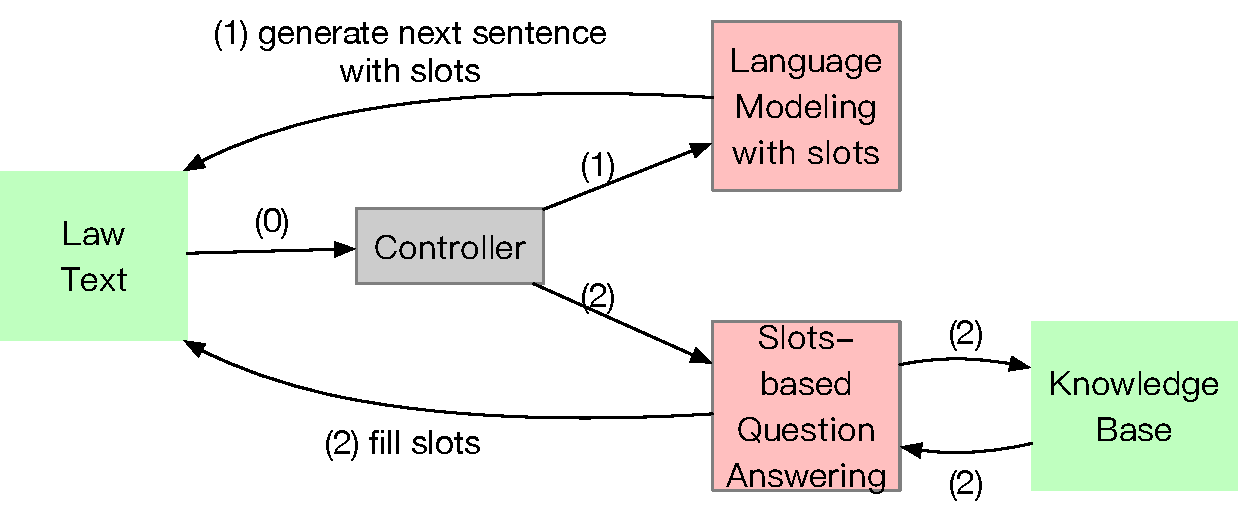
\includegraphics[width=1.0\columnwidth]{img/overall_architecture.pdf} 
\caption{Overall Architecture of CoLMQA.}
\label{fig:overall_architecture} 
\end{figure}

\begin{controlrule}[LM]
If  there's no slot in existing text, call LM to generate next sentence.
\end{controlrule}

\begin{controlrule}[QA]
If there are slots in existing text, call QA to fill slots. 
\end{controlrule}

\begin{controlrule}[End]
If there's an END symbol in existing text, finish the generation. 
\end{controlrule}

\subsection{Generating Texts with Slots by Language Modeling}
As shown in Figure \ref{fig:generation}, there are two phases in using a language model to generate texts with slots. 
The first phase is fine-tuning.
In this phase, after replacing the corresponding values in the original text with slots, we put the legal documents into a pre-trained model for fine-tuning, where different slots occupy different positions in the vocabulary. 

\begin{figure}[!htbp]
\centering 
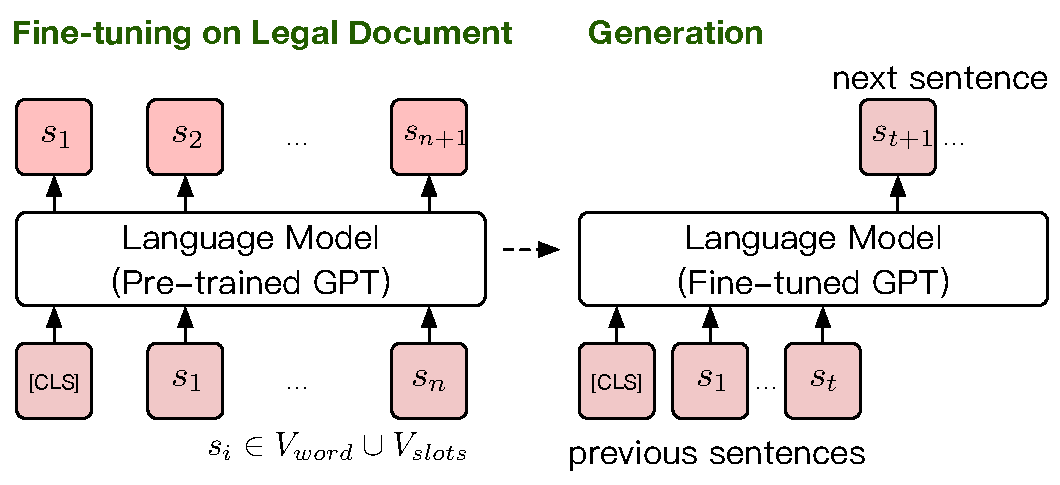
\includegraphics[width=1.0\columnwidth]{img/generation.pdf} 
\caption{Generation of texts with slots.} 
\label{fig:generation} 
\end{figure}

The second phase is to use the fine-tuned language model to generate texts with slots. 
We choose GPT as the language model in our work. 
So $V_{words}$ is the original vocabulary used by the pre-trained GPT, and $V_{slots}$ includes the additional placeholders in the fine-tuned GPT. 

\subsection{Filling Slots by Transformer-based Key-value Memory Networks}
\label{sec:TKVMemNN}
Briefly, our proposed method is in a family of Key-Value Memory Networks \cite{miller2016kvmemnn,das-etal-2017-textkbqa,xu2019enhancing}, but enhanced by Transformer encoder. 
As Xu~\shortcite{xu2019enhancing} pointed out, the standard Key-Value Memory Networks contain the following components: key hashing, key addressing, value reading, query updating, and answer prediction, which also applies in our proposed method. 
And in the above components, the standard KV-MemNNs exploit the bag of words to encode queries, keys, values, and candidate answers. 
This straightforward approach is not appropriate to encode very long queries key-value pairs stored in the Legal Knowledge Base, as shown in a running example in Figure \ref{fig:running_example}. 

\begin{figure}[!htbp]
\centering 
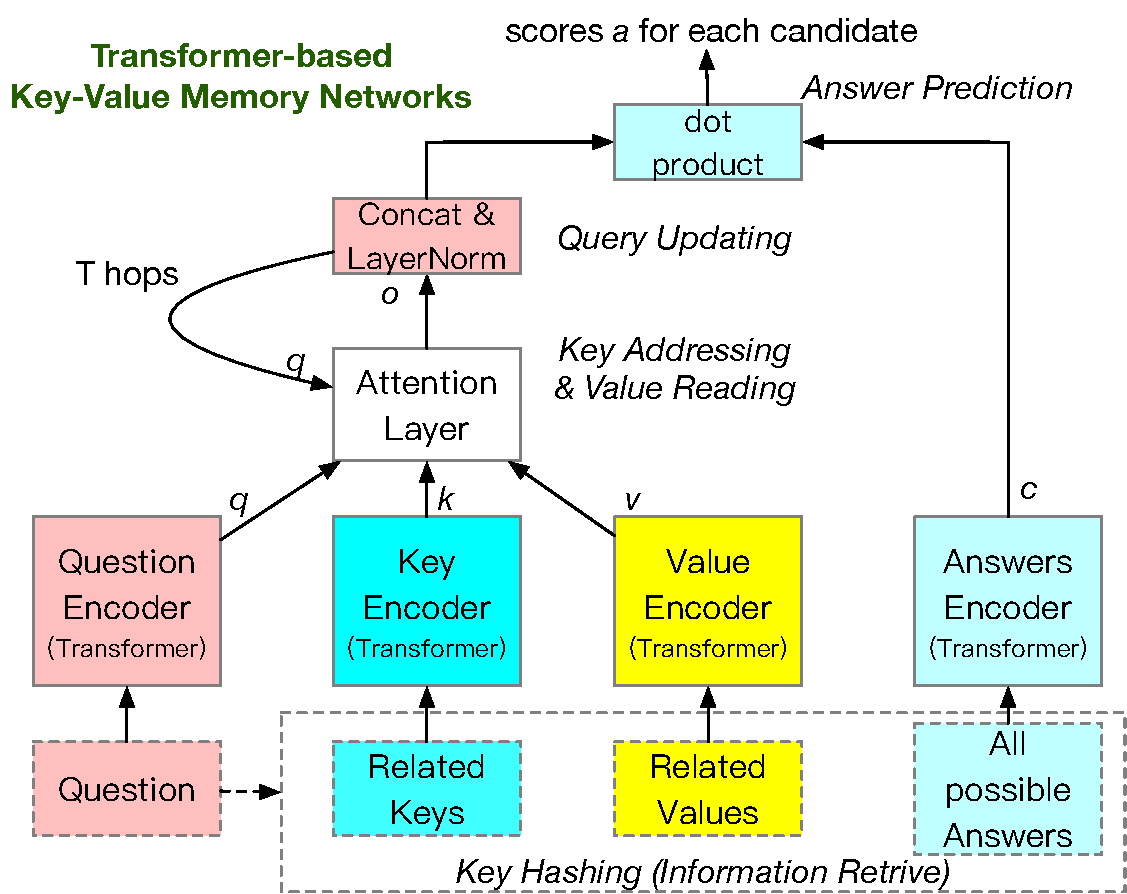
\includegraphics[width=1.0\columnwidth]{img/TKVMemNN.pdf} 
\caption{The illustration of the Transformer-based key-value memory networks, a KB enhanced QA method for filling slots.}
\label{fig:tkvmemnn} 
\end{figure}

\paragraph{Encoders.} 
Transformer has shown its ability to capture the long-range dependencies in natural language in GPT~\cite{radford2018improving} and BERT~\cite{devlin2019bert}. 
So rather than encoding the input as a bag of words, we use Transformer. 
We append a special token, i.e., [CLS], at the tail of a sentence $s$, then input it into an encoder with $n$ layer of Transformer encoder blocks. 
And then we use [CLS]'s corresponding output embedding $enc_{[\text{CLS}]}$ to represent the sentence $s$, and denote $Transformer(s) = enc_{\text{[CLS] in }s}$.


Since the Transformer encoder are pre-trained on all queries, keys, values, and candidate answers with an autoregressive task of predicting next words, the encoding of [CLS] can not be directly used in the Question Answering task. 
So we apply a linear projection $W_{\text{LHS}}\in \mathbb{R}^{H\times H}$ on $Transformer(s)$, where $H$ is the hidden size of Transformer encoder.

Equation (\ref{eq:question_encoder}) defines the Question Encoder in Figure \ref{fig:tkvmemnn}, given the original query $q$ as the input, to get the representation $q^{(0)}$ as the output. 
And all encoders in Figure \ref{fig:tkvmemnn} use a same Transformer.  
\begin{equation}
q^{(0)} = W_{\text{LHS}} \cdot \text{Transformer}(q)
\label{eq:question_encoder}
\end{equation}

\paragraph{Key hashing.} 
This component searches on the whole Legal Knowledge Base and gets query-related key-value pairs by conventional IR methods, e.g., TF-IDF or SQL selection on specific fields. 
Because the IR method doesn't go deeper into the sentence-level semantics of the query, and key-value pairs, we need to store them in memory and do re-organization by the remaining components.

\paragraph{Key addressing and value reading.}  
Key addressing reflects the relatedness between keys and query, as shown in Equation (\ref{eq:relatedness}) and Equation (\ref{eq:normalized_relatedness}). 
Similar to the scaled dot-product attention in Transformer, we rescaled the relatedness score $p^{(t)}$ with a factor of $1/\sqrt{H}$ when doing normalization. 
The superscript $t$ indicates the $t$-th hop (iteration) in multi-hop reasoning, and no more than the number $T$ of total hops.
\begin{equation}
p^{(t)}_i = (q^{(t)})^\top (W_{\text{LHS}} \cdot \text{Transformer}(k_i))
\label{eq:relatedness}
\end{equation}
\begin{equation}
\tilde{p}^{(t)}_i = \frac{\exp{(p^{(t)}_i/\sqrt{H} )}}{ \sum_{j} \exp{(p^{(t)}_j/\sqrt{H} )} }, \text{ for all}\ i
\label{eq:normalized_relatedness}
\end{equation}

Value reading is given by Equation (\ref{eq:value_reading}), summing the weighted encodings of values. 
\begin{equation}
o^{(t)} = \sum_{i} \tilde{p}^{(t)}_i \cdot W_{\text{LHS}} \cdot \text{Transformer}(v_i)
\label{eq:value_reading}
\end{equation}

Essentially, key addressing and value reading implements an attention layer to select which values are used to answer the query $q^{(t)}$. 

\paragraph{Query updating.} 
In the case of multi-hop reasoning, the query needs to be updated after each hop of reading on KB, because the newly read-in values should also be treated as a part of the query. 
In the running example in Figure \ref{fig:running_example}, the query is to ask which law and article number applies to the fact of misappropriating in a company. 
After one hop, the fourth value in Figure \ref{fig:running_example} could answer the question. 
But in a more complex situation, such as the misappropriating in a bank, one hop is not enough because Article 185 also refers to Article 272. 

%\begin{figure}[!htbp]
\begin{figure}
\centering 
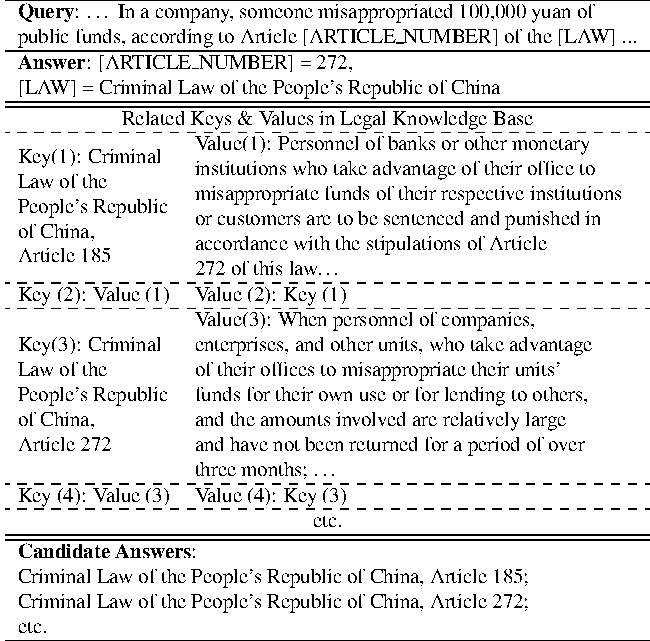
\includegraphics[width=1.0\columnwidth]{img/case.pdf} 
\caption{A running example of filling slots with KB enhanced QA. The slots of [ARTICLE\_NUMBER], [LAW], and their context are treated as the query. The values of slots are the answer. In this example, the fact of misappropriating in a company leads to Article 272 as the answer instead of Article 185, because the latter is about the misappropriating in banks or other monetary institutions.}
\label{fig:running_example} 
\end{figure}


We concatenate the query representation $q^{(t)}$ and the representation of related values $o^{(t)}$, then map to the $H$ dimension space by the matrix $M^{(t)} \in \mathbb{R}^{H\times 2H}$ to be a new query $q^{(t+1)}$.
\begin{equation}
q^{(t+1)} = \text{LayerNorm}( M^{(t)} \cdot (q^{(t)} \oplus o^{(t)} ))
\end{equation}


\paragraph{Answer prediction.} 
Rather than picking up all keys in Legal Knowledge Base $\mathcal{K}$ as candidate answers like TextKBQA~\cite{das-etal-2017-textkbqa}, we only conduct the similarity computation between $q^{(T)}$ and the retrieved candidates by Equations (\ref{eq:answer_prediction}) and (\ref{eq:softmax_normalization}). 
\begin{equation}
a^{(T)}_i = (q^{(T)})^\top \cdot W_{\text{RHS}} \cdot \text{Transformer}(c_i), \text{ for i-th candidate}
\label{eq:answer_prediction}
\end{equation}
\begin{equation}
\hat{y}^{(T)} = \text{softmax}(a^{(T)})
\label{eq:softmax_normalization}
\end{equation}

Considering the article number and law in $\mathcal{K}$ plays three roles in the network, such as the keys, the values, and the answers, we use a different matrix $W_{\text{RHS}}$ to do the necessary decoupling in Equation (\ref{eq:answer_prediction}).
Finally, the loss of cross-entropy between the prediction score $\hat{y}^{(T)}$ and the ground truth $y$ is taken for training the Transformer-based key-value memory networks. 
\begin{equation}
Loss(\hat{y}^{(T)}, y) = - \sum_{i} y_i \log \hat{y}^{(T)}_i
\end{equation}

\section{Empirical Study}
In this section, we demonstrate the effectiveness of our proposed method CoLMQA in the following aspects.
(1) We evaluate the quality of the generated texts with slots to show the language model is capable of predicting the number of slots and the composition of slots and words, which is critical to our divide-and-conquer strategy. 
(2) Comparing to other QA methods, we test the accuracy of filling slots by our proposed Transformer-based key-value memory networks. 

\subsection{Legal Document Dataset and Legal Knowledge Base}
\label{sec:legal_documents}
\paragraph{Legal Document Dataset.} 
All the experiments are conducted on the judicial documents from China Judgements Online\footnote{\url{http://wenshu.court.gov.cn/}}, which are widely used in NLP works in legal domain~\cite{luo2017learning_charge,ye-etal-2018-interpretable_courtviews}. 
We crawled 11,327,945 judicial documents from China Judgements Online in 2015. 
The legal documents cover diverse branches of law. 
For instance, we tokenized the document titles with a Chinese Tokenizer jieba\footnote{\url{https://github.com/fxsjy/jieba}}, and do the quick overview of the wordcount, then find out that the word \textit{"dispute"} appearing in 4,774,968 (42.1\%) document titles, the word \textit{"limited company"} 30.5\%, the word \textit{"criminal"} 17.2\%, and the word \textit{"divorce"} 8.5\%, etc. 

We randomly select 20,000 documents from the dataset, splitting to the training data, validation data, and testing data, with the portion 80\%, 10\%, and 10\%. 
By regular expressions, the fact descriptions, and court views are extracted. 
We mainly consider the generation of court views, which is the explanation for the charge. 
And court views contain the applicable law article to make the charge interpretable. 

\paragraph{Legal Knowledge Base.} 
We collect the required legislative documents according to the law articles mentioned in the legal document dataset, e.g., the Criminal Law of the People's Republic of China. 
On the basis of the collected legislative documents, the regular expression and a finite-state machine are used to extract the (key, value) pairs, where the key represents law article and value represents the detailed content. 
In the end, the Legal Knowledge Base is built upon the 149 laws, civil codes, and interpretations, which appeared in the aforementioned Legal Document Dataset. 

\subsection{LM with Slots}
\paragraph{Slots}
Based on the level of uncertainty, we modeled 7 slots: [NAME], [DATE], [MONEY], [ADDRESS], [NUMBER], [LAW], [ARTICLE\_NUMBER].
We use the regular expression to replace the values in court views part in legal documents with the above slot placeholders.
The first five slots reduce the uncertainty of language modeling. 
The last two slots correspond to two parts of a law article, which are the law's name and the number pointing to the law article. 
They have specific values in our built Legal Knowledge Base. 
These values can be obtained by reasoning based on the text content. 
Therefore, they are within the consideration of slot filling in our question-answering model.
And we denote the first five slots as the Type A slots and the last two slots as the Type B slots. 
The Type A slots used here is to demonstrate that language models can benefit from reducing the uncertainties when generating text, especially when they don't have to predict the exact number of [MONEY] or the value of [DATE].  

\paragraph{Language models with(out) slots.} 
Language Models are categorized into different groups depending on whether trained with slots or without slots as shown in Table \ref{tbl:slots_accuracy}. 
We use two versions of GPT\footnote{\url{https://github.com/huggingface/transformers}}, pre-trained, and without pre-trained. 
The former is pre-trained on a news dataset\footnote{It's news2016zh dataset in \url{https://github.com/brightmart/nlp_chinese_corpus}.} which contains 2.5 million news articles for one epoch on a 4$\times$ NVIDIA Tesla V100 machine, and with the stride being 768. 
The sequence length of the Transformer block used in both GPT versions is 1024.
The text generation sub-task is given a prompt (the facts part in a judicial document), then to generate a sentence by using the Beam search. 

\begin{table}[]
\scalebox{0.88}{
\begin{tabular}{c|c|c|c|c}
\hline
 & \begin{tabular}[c]{@{}c@{}}without\\ slots\end{tabular} & \multicolumn{1}{c|}{\begin{tabular}[c]{@{}c@{}}with\\ Type A slots\end{tabular}} & \begin{tabular}[c]{@{}c@{}}with\\ Type B slots\end{tabular} & \begin{tabular}[c]{@{}c@{}}with\\ all slots\end{tabular} \\ \hline
RNN & 0.131 & 0.198 & 0.186 & 0.292 \\ \hline
GPT & 0.238 & 0.441  & 0.425 & 0.573 \\ \hline
\begin{tabular}[c]{@{}c@{}}GPT\\ (pre-trained)\end{tabular} & 0.421 & 0.642 & 0.573 &  0.682 \\ \hline
\end{tabular}
}
\caption{The F score of predicting law article slots (Type B slots) of different language models, on test dataset.}
\label{tbl:slots_accuracy}
\end{table}


\begin{table}[]
\scalebox{0.9}{
\begin{tabular}{c|c|c|c|c}
\hline
 & \begin{tabular}[c]{@{}c@{}}without\\ slots\end{tabular} & \begin{tabular}[c]{@{}c@{}}with\\ type A slots\end{tabular} & \begin{tabular}[c]{@{}c@{}}with\\ type B slots\end{tabular} & \begin{tabular}[c]{@{}c@{}}with\\ all slots\end{tabular} \\ \hline
RNN & 67.9 & 59.6 & 62.8 & 53.1 \\ \hline
GPT & 12.8 & 10.3 & 11.9 & 8.2 \\ \hline
\begin{tabular}[c]{@{}c@{}}GPT\\ (pre-trained)\end{tabular} & 11.3 & 8.8 & 10.5 & 7.8 \\ \hline
\end{tabular}
}
\caption{The perplexity on test dataset. }
\label{tbl:slots_perplexity}
\end{table}



%\paragraph{The accuracy of predicting on law article slots.} 
\paragraph{Result.} 
In the first sub-task, after removing some highly uncertain content and replacing it with slots, the language model can generate more deterministic text and make the sentence more fluent as shown in Table \ref{tbl:slots_accuracy} and Table \ref{tbl:slots_perplexity}.

Given a prompt, we use a language model to generate the court view that contains slots and then count the generated Type B slots in it. 
The F score in Table \ref{tbl:slots_accuracy} is computed between two Type B slot sequences by matching one by one. 
As a toy example, a ground truth in a court view containing slots like \textit{"in accordance with Article b and Article b of a"}, where a=[LAW], b=[ARTICLE\_NUMBER], and the slot sequences in a generated text is like \textit{"in accordance with Article b of a, Article b of a, and Article b of a"}. 
Then the precision of predicting Type B slots ([LAW] and [ARTICLE\_NUMBER]) is 1/6 because the first one slots are matched one by one, while the recall of predicting Type B slots is 2/3 when considering the total length of subsequences \textit{"b*a"} in the ground truth is matched by the generated sequence. 
The F score in this toy example is 0.27. 
In this way, the F score is used to measure how good the text sequence with slots is matched to the ground truth.
When computing the F score of the slots prediction by using the model without slots, we do a manual conversion to replace the values with slots in the result.

In Table \ref{tbl:slots_accuracy}, we compare different language models and different settings and find out that the pre-trained GPT can effectively generate a sentence with correct slots.
In Table \ref{tbl:slots_perplexity}, the perplexity on the test dataset demonstrates that the generated sentence of the court view is fluent when considering slots. 


\subsection{Filling Slots by Transformer-based Key-Value Memory Networks}
\paragraph{Construction of query-answer pairs.} 
To derive the query-answer training pairs from the Legal Document Dataset in Subsection \ref{sec:legal_documents}, we consider different situations as follows.
 
The first one is that a court view part in the legal judicial document only contains one applicable law article in the form of "According to Article 263 of the Criminal Law of ...". 
In this case, the query in a query-answer pair is the text span from the beginning to the position of current law article, while the value is the ground truth, e.g., Article 263 of the Criminal Law. 
The second one is that a court view contains more than one applicable law article with the same law, such as "According to Article 263 and Article 269 of the Criminal Law". 
In this one, we make multi tiny-modified copies, Query1: "According to [ARTICLE\_NUMBER] of the [LAW]", Query2: "According to Article 263 and [ARTICLE\_NUMBER] of the Criminal Law". 
The third one is the mixing case, that different laws and different law articles are cited in a court view, which can be processed like the second one.  
On average, there are 4.1 query-answer pairs produced per court view. 
And the average length of a query is 2783. 
For the query which is longer than the sequence length of Transformer Encoder in TKVMemNN, we keep the tail part of the query sequence, which is reasonable as the fact description appears more often in the tail part.

\paragraph{Training of our method.} 
We use the first four layers of Transformers in our pre-trained GPT as the encoder for queries, keys, values, and answers in the experiment, then carry out the two-phases fine-tuning. 
The first-phase fine-tuning is conducted on the task of predicting the next words in the sequences of queries, keys, and values. 
The second-phase fine-tuning is training the proposed model TKVMemNN on our constructed query-answer pairs and the Legal Knowledge Base. 
To conduct the multi-hop reasoning, we set the number of hops $T$ as 3. 
\paragraph{Baselines.} We use Whoosh (a Python IR open-source toolkit), Memory Networks, and their variants with or without the document title as baselines. 
As the title are important for providing additional information, such as the type of documents, they are useful for filling slots. 
 
Because the computation of the dot product between the query and the encodings of all the candidates in the Legal Knowledge Base is very expensive, we limit the number of candidates in IR scope to improve the efficiency. 

\begin{table}[h]
\scalebox{0.88}{
\begin{tabular}{c|c|c|c|c}
\hline
MemNN & Whoosh & \begin{tabular}[c]{@{}c@{}}Whoosh\\ +title\end{tabular} & TKVMemNN & \begin{tabular}[c]{@{}c@{}}TKVMemNN\\ +title\end{tabular} \\ \hline
0.23 & 0.13 & 0.17 & 0.39 & 0.41 \\ \hline
\end{tabular}
}
\caption{The accuracy of filling slots.}
\label{tbl:accuracy_filling_slots}
\end{table}


\paragraph{Result.} 
In the second sub-task, the multi-hop reasoning on the knowledge base makes the generated text more logical as illustrated in Table \ref{tbl:accuracy_filling_slots}.

\section{Conclusion and Future Works}
In order to solve the problem of conflicting logics appeared in the text generated by a language model, we propose a novel method CoLMQA which benefits from Language Modeling and Question Answering simultaneously. 
In the Language Modeling component, the sentences with slots are generated and provided a well-written skeleton of sentences. And in the Question Answering component, the slots are filled with accurate values with the help of Knowledge Base. 
In our experiment, we verified that our method can fill slots with logical coherent values. 
In the future, we'll expand CoLMQA to other scenarios of text generation which also require keeping logic, but using different kinds of slots. 

\section*{Acknowledgments}
We thank Xi Chen, Ni Li, Yan Cui, Mingkuo Ji, Jun Chen, Yuren Wu, and Hanzhang Yang for helpful discussions.

%% The file named.bst is a bibliography style file for BibTeX 0.99c
\bibliographystyle{named}
\bibliography{ijcai20}

\end{document}

